\chapter{TEORI DASAR}
\vspace{1.0cm}

%-----------------------------------------------------------------------------%
\section{Teori ke-1}
%-----------------------------------------------------------------------------%
Lorem ipsum dolor sit amet, odio utroque definiebas ut quo, delenit omittam ne nec. Ius in assentior consectetuer, eos id malorum prodesset accommodare. Quot explicari definitionem eam eu, magna adipiscing eu nec. Dicta dicam sanctus vis cu, vel ne autem civibus facilisis. Ad dicat dolores pro, sea ex wisi justo possim, alienum reprehendunt vim ad. Sed quas verear ea, et wisi timeam percipitur his. Probo scaevola vim cu. Ea vix assum recusabo, fabulas maiestatis ei sed. Pri wisi omnesque ex. Eum ea mundi laoreet appellantur, postea vidisse efficiantur sed ad. Duo case civibus ea, no pro recusabo scripserit. Has id audire deterruisset. Eam cu cibo exerci, et facilisis consetetur vix, mel an soleat ceteros. Ex prima eirmod vulputate pri, eum no essent mandamus. Albucius accusamus salutatus vix at, assum ullamcorper ex sea. Vis eleifend consetetur ut, ex ius verear rationibus sadipscing. Meliore assentior sit cu. Vidisse omittantur vim ne. Regione accusam vituperatoribus vel ut, et sit commodo concludaturque. (lihat Gambar \ref{fig:garputala}). \\
\begin{figure}[H] 
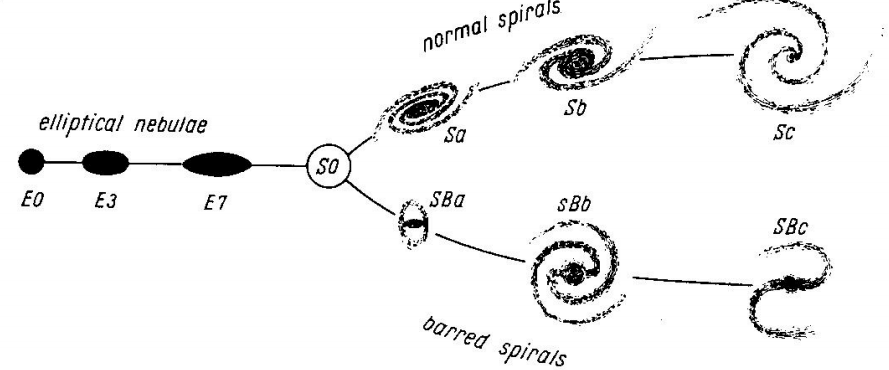
\includegraphics[scale=0.45]{pics/garputala.png}
\caption[Diagram garpu tala Hubble]{Diagram garpu tala Hubble yang menunjukkan klasifikasi galaksi elips, spiral, dan lentikular (Sumber: Hubble, 1958)}
\label{fig:garputala}
\centering
\end{figure}
	Lorem ipsum dolor sit amet, odio utroque definiebas ut quo, delenit omittam ne nec. Ius in assentior consectetuer, eos id malorum prodesset accommodare. Quot explicari definitionem eam eu, magna adipiscing eu nec. Dicta dicam sanctus vis cu, vel ne autem civibus facilisis. Ad dicat dolores pro, sea ex wisi justo possim, alienum reprehendunt vim ad. Sed quas verear ea, et wisi timeam percipitur his. Probo scaevola vim cu.\\
	
	Ea vix assum recusabo, fabulas maiestatis ei sed. Pri wisi omnesque ex. Eum ea mundi laoreet appellantur, postea vidisse efficiantur sed ad. Duo case civibus ea, no pro recusabo scripserit. Has id audire deterruisset. Eam cu cibo exerci, et facilisis consetetur vix, mel an soleat ceteros.\\
	
	Ex prima eirmod vulputate pri, eum no essent mandamus. Albucius accusamus salutatus vix at, assum ullamcorper ex sea. Vis eleifend consetetur ut, ex ius verear rationibus sadipscing. Meliore assentior sit cu. Vidisse omittantur vim ne. Regione accusam vituperatoribus vel ut, et sit commodo concludaturque.\\
	
\begin{figure}[H] 
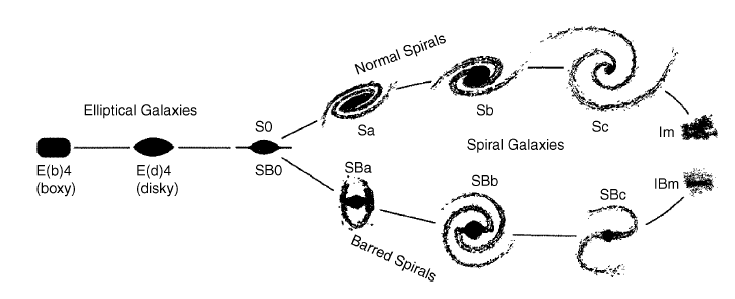
\includegraphics[scale=0.55]{pics/garputala2.png}
\caption[Diagram garpu tala Hubble hasil modifikasi]{Diagram garpu tala Hubble yang dimodifikasi, yang mengklasifikasikan galaksi menjadi galaksi elips, lentikular, spiral dan iregular (Sumber: Schneider,  2010)}
\label{fig:garputala2}
\centering
\end{figure}
%-----------------------------------------------------------------------------%
\section{Fotometri Galaksi Spiral}
%-----------------------------------------------------------------------------%
\subsection{Fotometri Galaksi}
%-----------------------------------------------------------------------------%
Lorem ipsum dolor sit amet, odio utroque definiebas ut quo, delenit omittam ne nec. Ius in assentior consectetuer, eos id malorum prodesset accommodare. Quot explicari definitionem eam eu, magna adipiscing eu nec. Dicta dicam sanctus vis cu, vel ne autem civibus facilisis. Ad dicat dolores pro, sea ex wisi justo possim, alienum reprehendunt vim ad. Sed quas verear ea, et wisi timeam percipitur his. Probo scaevola vim cu. \\

	Ea vix assum recusabo, fabulas maiestatis ei sed. Pri wisi omnesque ex. Eum ea mundi laoreet appellantur, postea vidisse efficiantur sed ad. Duo case civibus ea, no pro recusabo scripserit. Has id audire deterruisset. Eam cu cibo exerci, et facilisis consetetur vix, mel an soleat ceteros.

\begin{equation} \label{kecerlangan}
I=\dfrac{F}{\alpha^{2}}=\dfrac{\dfrac{L}{4 \pi d^{2}}}{\bigg(\dfrac{D}{d} \bigg)^{2}}=\dfrac{L}{4 \pi D^{2}}
\end{equation}
dengan  $F$ merupakan kecerlangan semu. $L$ merupakan luminositas galaksi dan $D$ merupakan luas galaksi yang diamati pada jarak $d$ dan sudut ruang $\alpha$. Untuk galaksi yang memiliki piringan datar, kecerlangan permukaan berbanding terbalik dengan $\cos i$, $I \propto \dfrac{1}{\cos i}$. \\

	